%===========================================================================================
\section{Detailed Description of the Merger Tree algorithm}\label{app:detailed_mergertree}
%===========================================================================================


The merger tree code starts once clumps have been identified and the particle unbinding is completed.
The algorithm is designed to work in parallel on distributed memory architectures and makes use of the MPI standard.
When \ramses\ is executed, each processing unit involved in the execution is typically referred to by a unique index, 
called the ``MPI rank'', and given a unique domain, i.e. part of the volume of the simulated space, to work on. 
In what follows, we assume that the code is being executed in parallel over multiple MPI ranks.
The code then proceeds as follows:

\begin{enumerate}
%	
	\item Write the current clump data to file which is to be read in as progenitor data in the subsequent snapshot:
		For every clump, identify up to $n_{mb}$ tracer particles with minimal binding energy.
		If a clump consists of less than $n_{mb}$ particles, then take the maximally available number of particles.
		Then write the tracer particles of all ranks into a single shared file. 
		This file will be read in by every rank in once the next snapshot is being processed.
		If past merged progenitors exist, each rank writes these to (a different) shared file for later use.

%		
%	
	\item Every rank reads in the progenitor data from the shared file of the previous snapshot.
	
	\item The read in progenitor data is processed:
		First we find which progenitor tracer particles are on each rank's domain by comparing the tracer particles' unique ID to the IDs of the particles currently in this rank's domain.
		Each rank needs to know which tracer particles are currently on its own domain.	
		Then we find and communicate globally which rank is the ``owner'' of which progenitor (and past merged progenitor): 
		The owner of any progenitor is defined as the rank which has the most strongly bound particle of that progenitor within its domain.
		This particle is referred to as the ``galaxy particle'' of this progenitor.
		Each rank henceforth only keeps track of the tracer particles that are on its domain.
		The rest are removed from memory.

	
	\item Find links between progenitors and descendants, that is find ``which tracer particle ended up where'':
	
		After clump finding, the clump to which any particle belongs is known, and after reading in progenitor data, the progenitor clump 
		to which any tracer particle belonged to is known.
		Each rank now loops through all its local tracer particles.
		Using these two informations (in which clump the particle was and in which clump the particle is now) for every tracer particle, 
		all descendant candidates for all progenitors are found and stored in a sparse matrix, where the rows of the matrix correspond 
		to progenitors and the columns are the descendants.
		The exact number of particle matches between a progenitor-descendant candidate pair is kept.
%		For example: let $n_{mb}=200$. For the progenitor with ID 1, a possible result would be to find 50 particles in descendant with ID 2, 120 particles in descendant with ID 7, 10 particles in descendant 3 and 20 particles that aren't in a clump at the current snapshot.
		
		With the sparse matrices populated, they are now communicated across ranks where they are needed. 
		First every rank that has data on progenitors that it doesn't own itself sends this data (specifically, the sparse matrix data) to the owner of that progenitor.
		The owners then gather and sum up all the matches found in the previous linking step for the progenitors that they own and then send them 
		back to any rank that has at least one particle of that progenitor on their domain.
		(These are the same ranks that sent data to the owner of the progenitor in the first place.)
		
		After communications are done, a transverse sparse matrix is created, where the rows are descendants and the columns are progenitors.
		These matrices will be used to loop through progenitor or descendant candidates.
		

	
	\item Make trees:
		We first obtain an initial guess for the main progenitors of every descendant and for the main descendant of every progenitor by
		finding the candidate that maximises the merit function given by Equation~\eqref{eq:merit}.
		
		Then we loop to establish matches:
		
		A main progenitor-descendant pair is established when the main progenitor of a descendant is the main descendant of said progenitor, or in pseudocode:
		\begin{verbatim}
		match = (main_prog(idesc)==iprog) && 
        (main_desc(iprog)==idesc)
		\end{verbatim}
		
		While there are still descendants without a match and still progenitor candidates left for these descendants:
		
		\begin{itemize}
			
			\item For progenitors without a match: Loop through all descendant candidates. 
					If you find a match, stop there and mark this descendant candidate as the main descendant for this progenitor.
			
			\item Then for all descendants still without a match: Switch to the next best progenitor candidate as current best guess.
			
		\end{itemize}
		
		The loop ends either when all descendants have a match, or if descendants run out of candidates.
		If a progenitor hasn't found a match at this point, we assume that it merged into its best descendant candidate, i.e. the one that maximises the merit function.
	  The merged progenitors are added to the list of past merged progenitors by adding their ``galaxy particle'' to the list.
		
		If there are descendants that still have no main progenitor, we now try finding a progenitor from an older, non-consecutive snapshot.
		Past merged progenitors are tracked by one particle, their former ``galaxy particle'', which we now refer to as the ``orphan particle''.
		All particles of the descendant under investigation are checked for being an orphan particle of a past merged progenitor.
		The most strongly bound orphan particle will be considered the main progenitor of the descendant under consideration.
		If a match is found, the past merged progenitor is removed from the list of past merged progenitors.
		
		Finally, descendants that still haven't found a progenitor at this point are deemed to be newly formed.
		
	\item The results are written to file.
	
	

	
\end{enumerate}

















%========================================================================================================
\section{Tree Statistics Using \citet{SUSSING_HALOFINDER} Selection Criteria}\label{app:performance_comparison}
%========================================================================================================



\begin{table}
\centering
\caption{
	Comparison of simulation and evaluation parameters used in this work and of A14, where the parameters of the latter have been converted using $h = 0.704$.
	$m_m$ is the mass threshold for main haloes, $m_s$ is the mass threshold for sub-haloes.
	\label{tab:parameter-comparison}
}
	\begin{tabular}[c]{l l l}
													&	This work		&	A14 \\
		\hline
		particle mass	[$10^9 \msol$]				&	$1.55$			& $1.32$						\\
		particles used								& 	$256^3$			& $270^3$ 						\\
		box size [Mpc]								& 	$88.6$			& $88.8$						\\
		snapshots until $z = 0$						&  	67				& 62							\\				
		$m_m$ [$10^{12} \msol$]						&	$1.51$			& $1.12$ - $1.37$				\\
		$m_s$ [$10^{11} \msol$]						&	$3.91$			& $4.26$ - $9.72$				\\
		\hline
	\end{tabular}
\end{table}


\begin{figure}
	\centering
	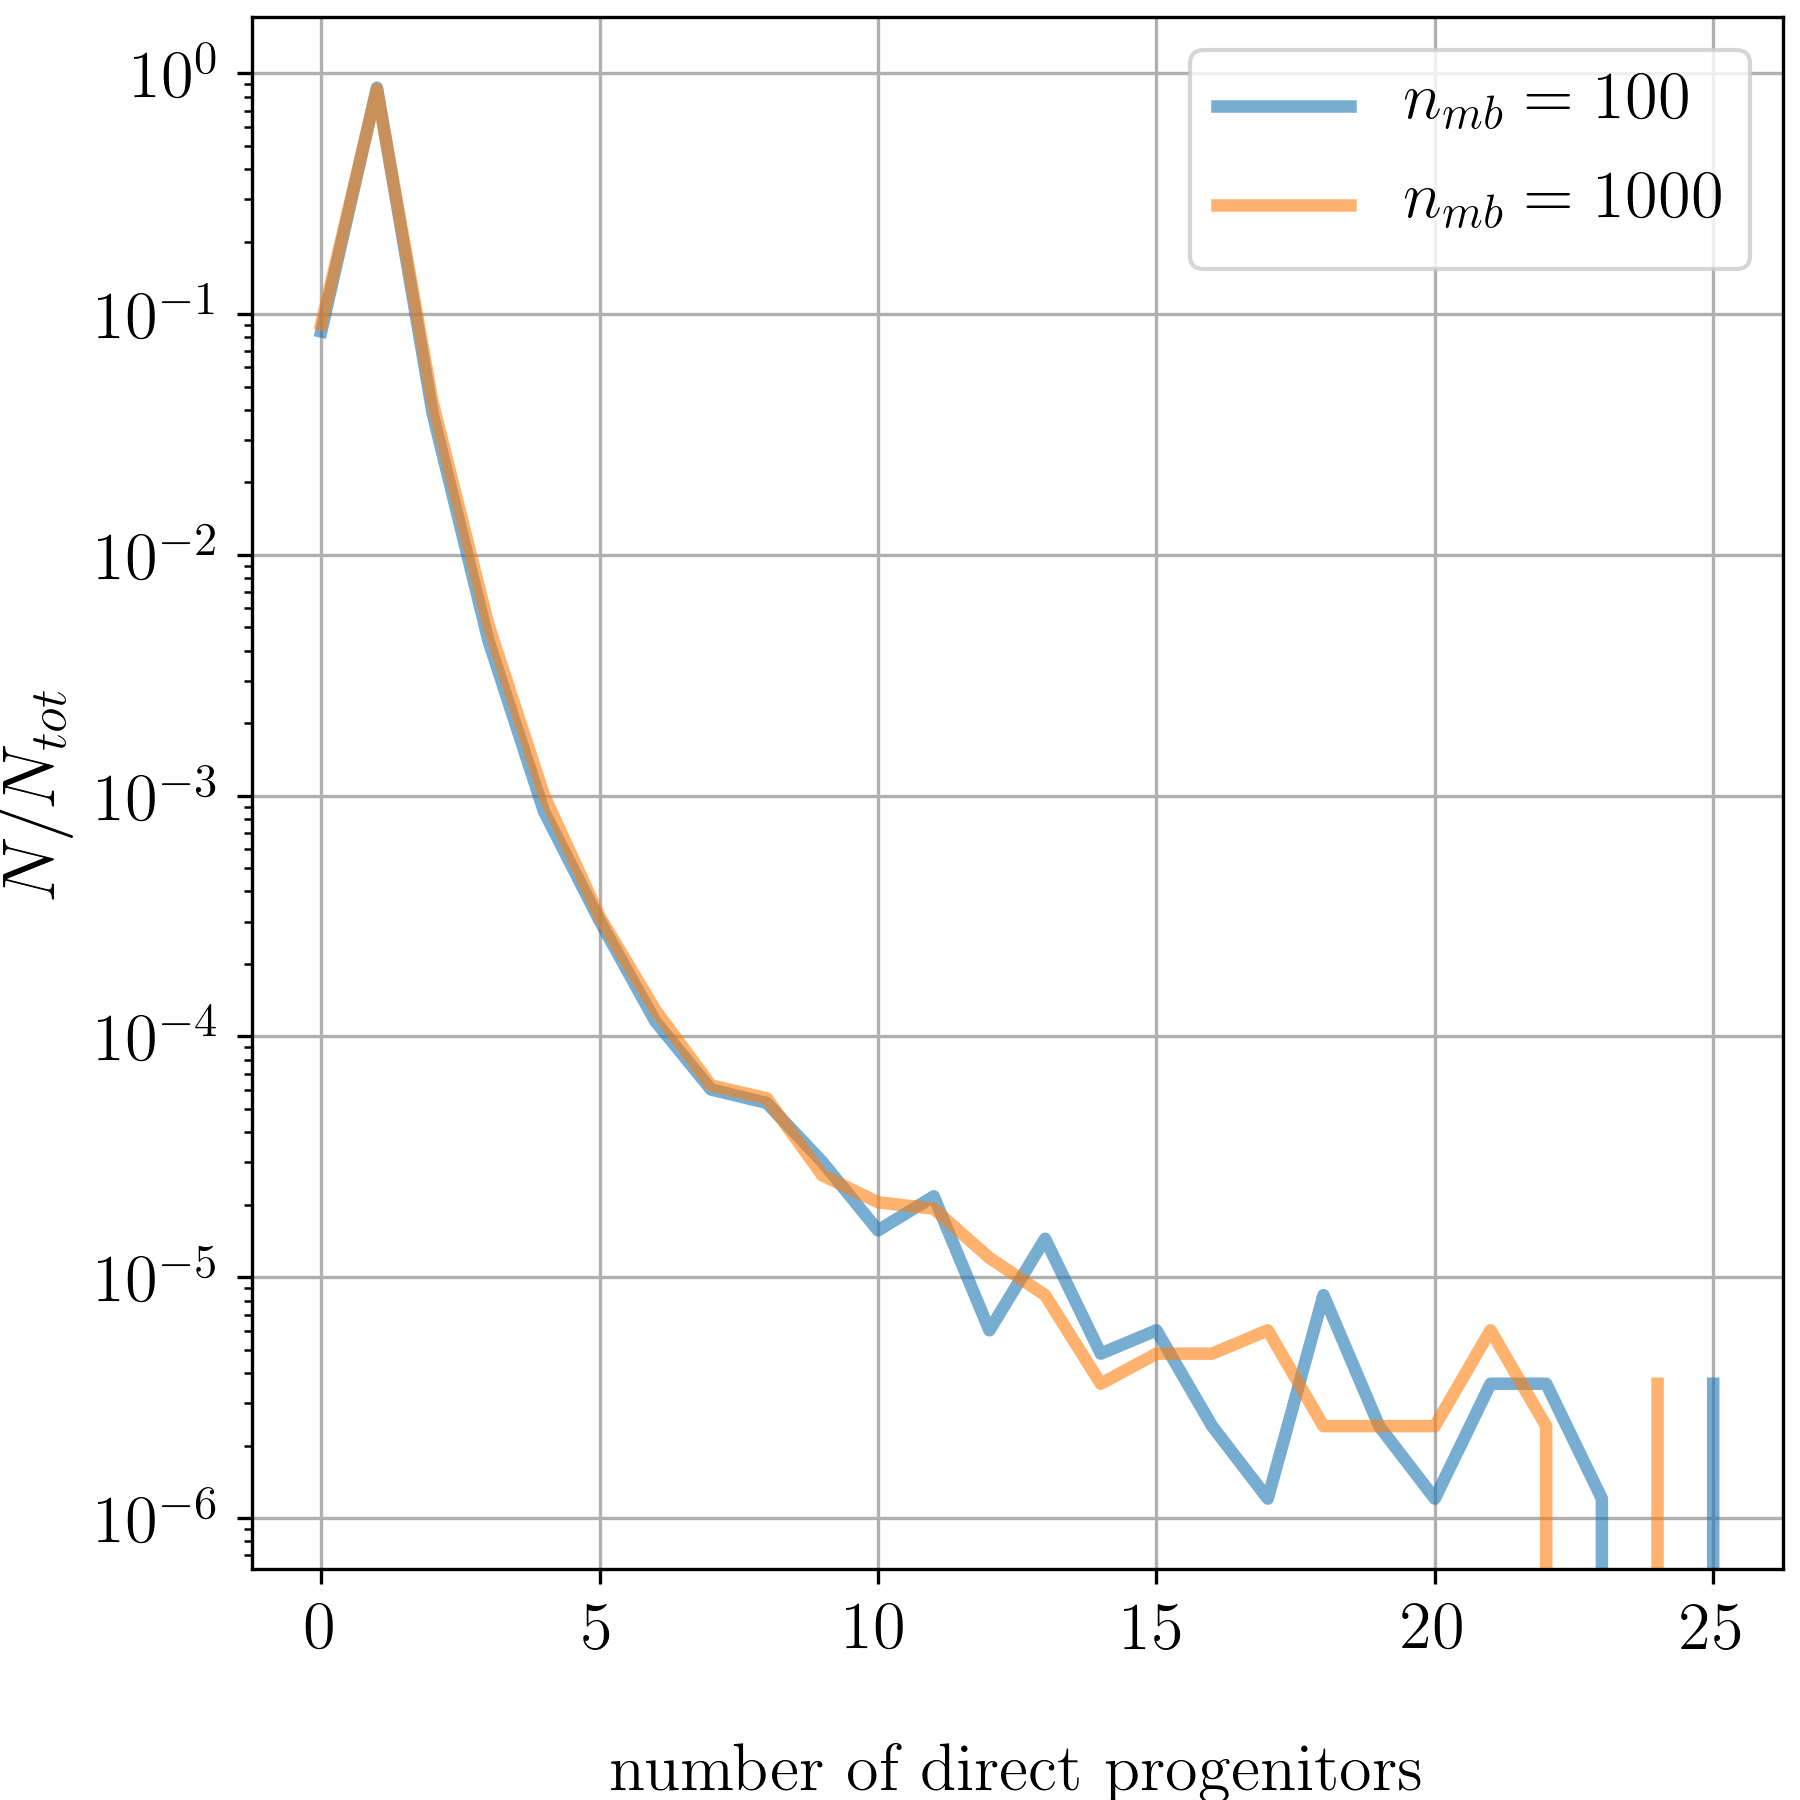
\includegraphics[width=.9\linewidth, keepaspectratio]{images/tree-statistics-sussing-threshold/branching-ratio-ntrace.png}\\%
	\caption{
		Histogram of the number of direct progenitors for all clumps from $z = 0$ to $z = 2$ for $n_{mb} = 100$ and $1000$ tracer particles per clump.
		The histogram is normalized by the total number of events found.
	}%
	\label{fig:sussing-branching-ratio}
\end{figure}

\begin{figure}
	\centering
	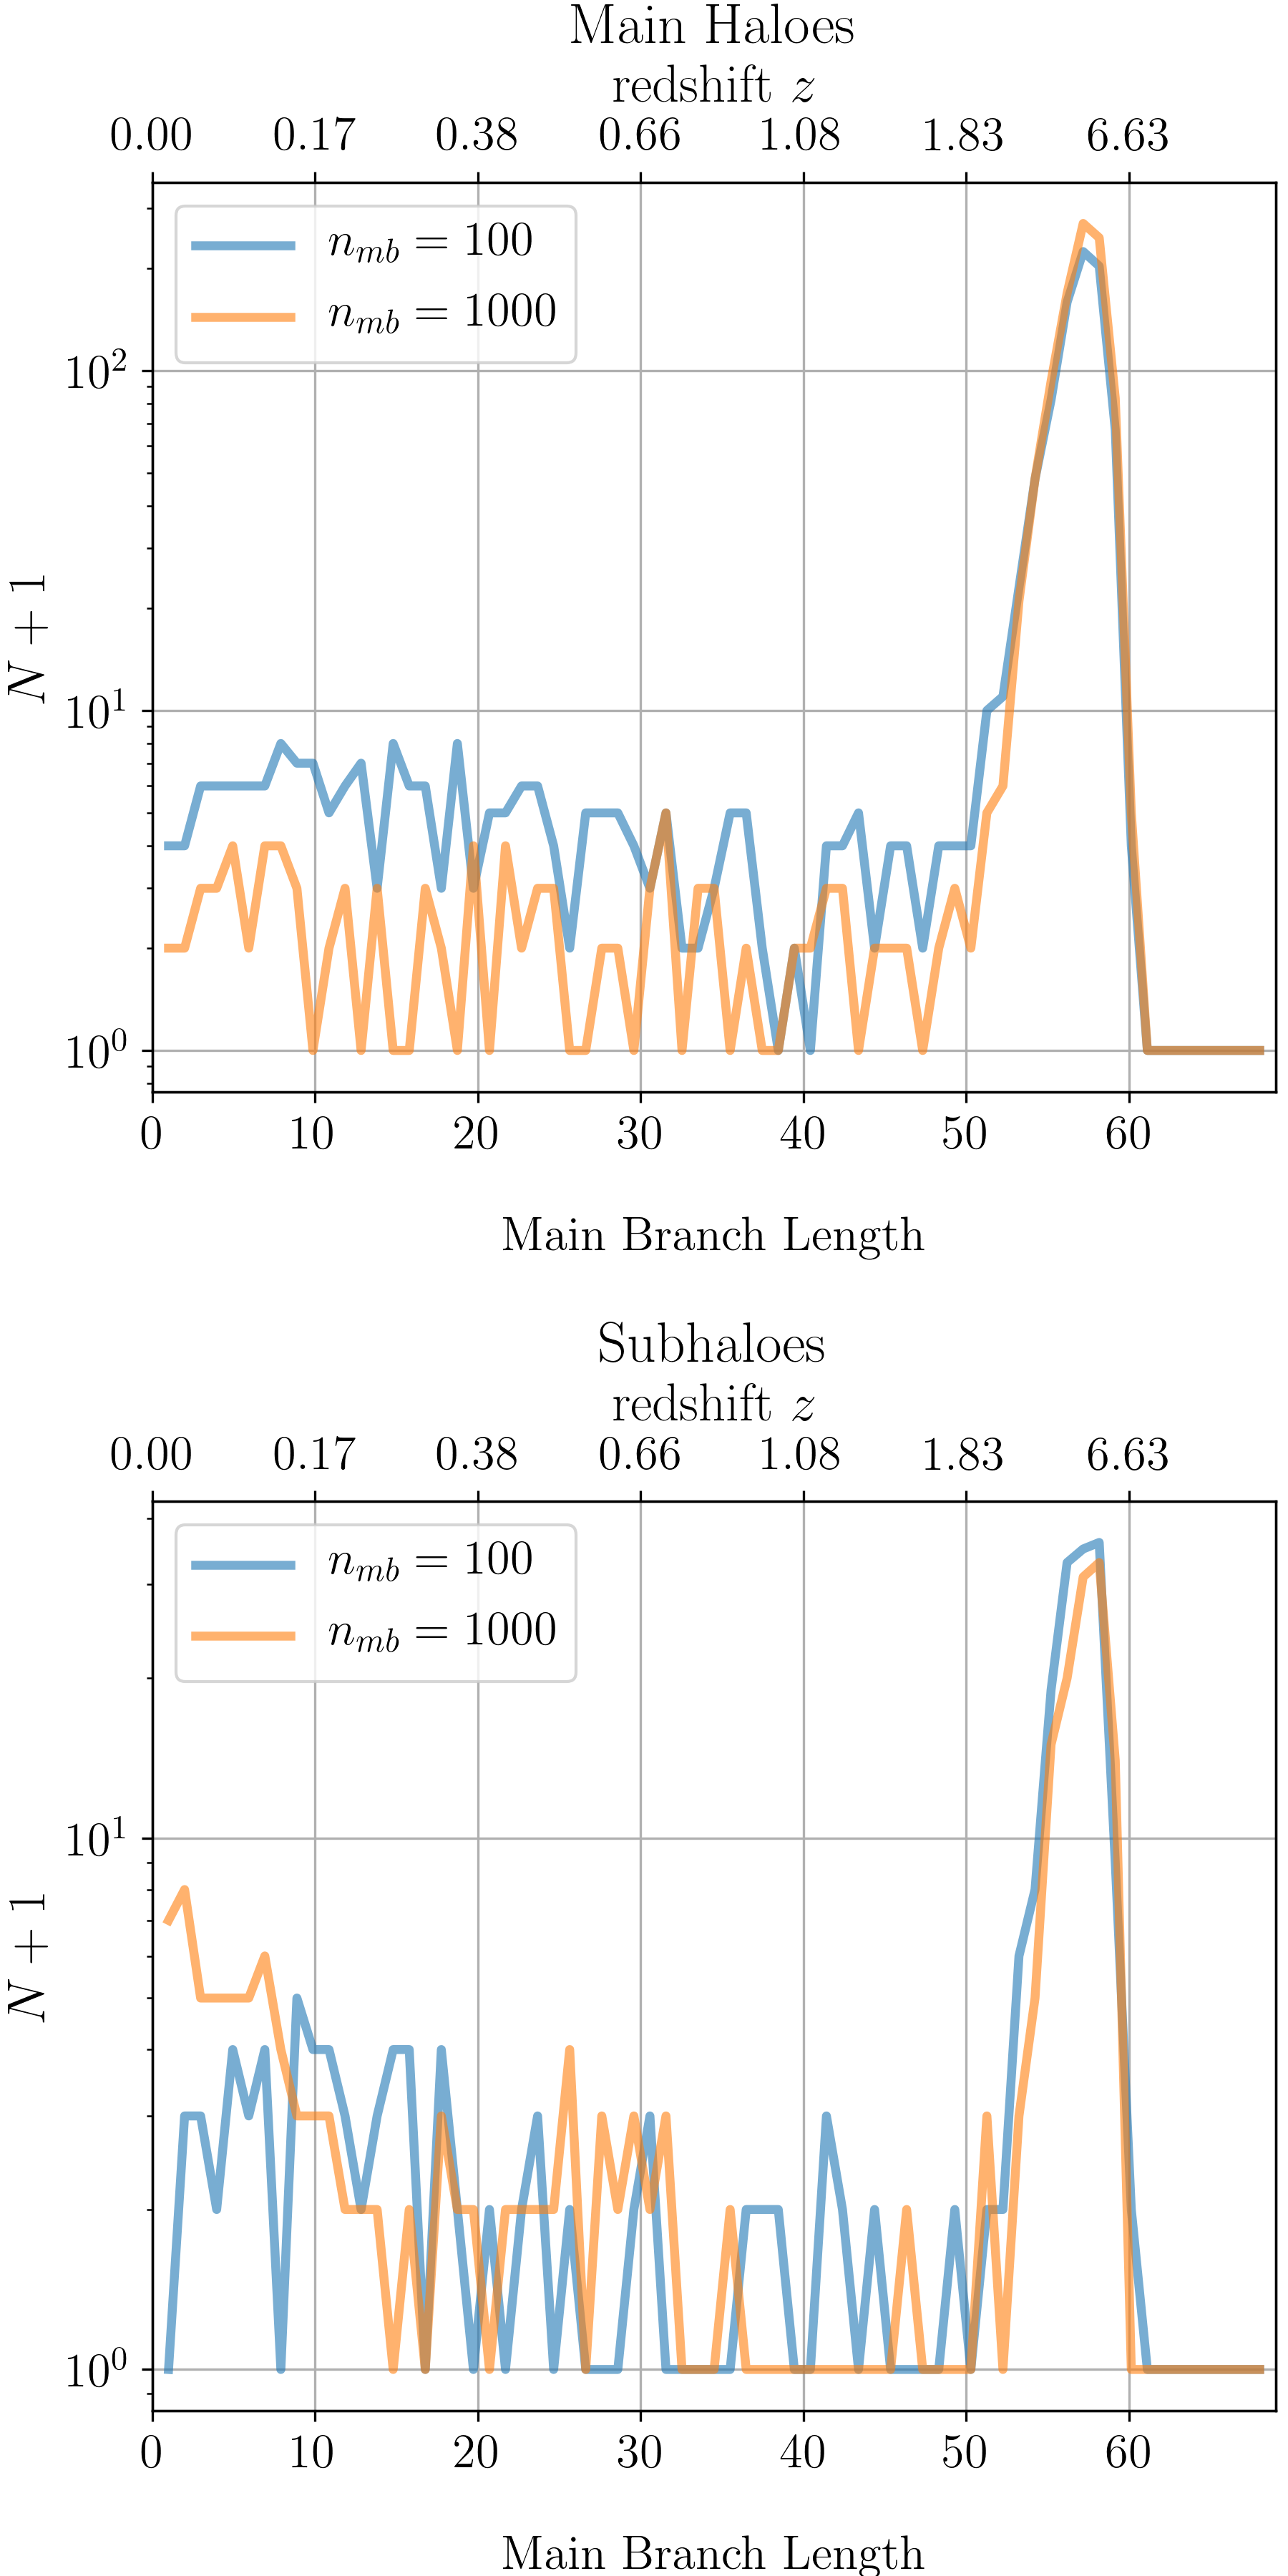
\includegraphics[width=.95\linewidth, keepaspectratio]{images/tree-statistics-sussing-threshold/main-branch-lenghts-all-bins-ntrace.png}%
	\caption{
		Histograms of the length of the main branch. 
		The left plot shows the length of the 1000 most massive haloes at $z = 0$, the right plot shows the length of the 200 most massive sub-haloes for $n_{mb} = 100$ and $1000$ tracer particles per clump.
	}%
	\label{fig:sussing-branch-lengths}
\end{figure}

\begin{figure*}
	\centering
	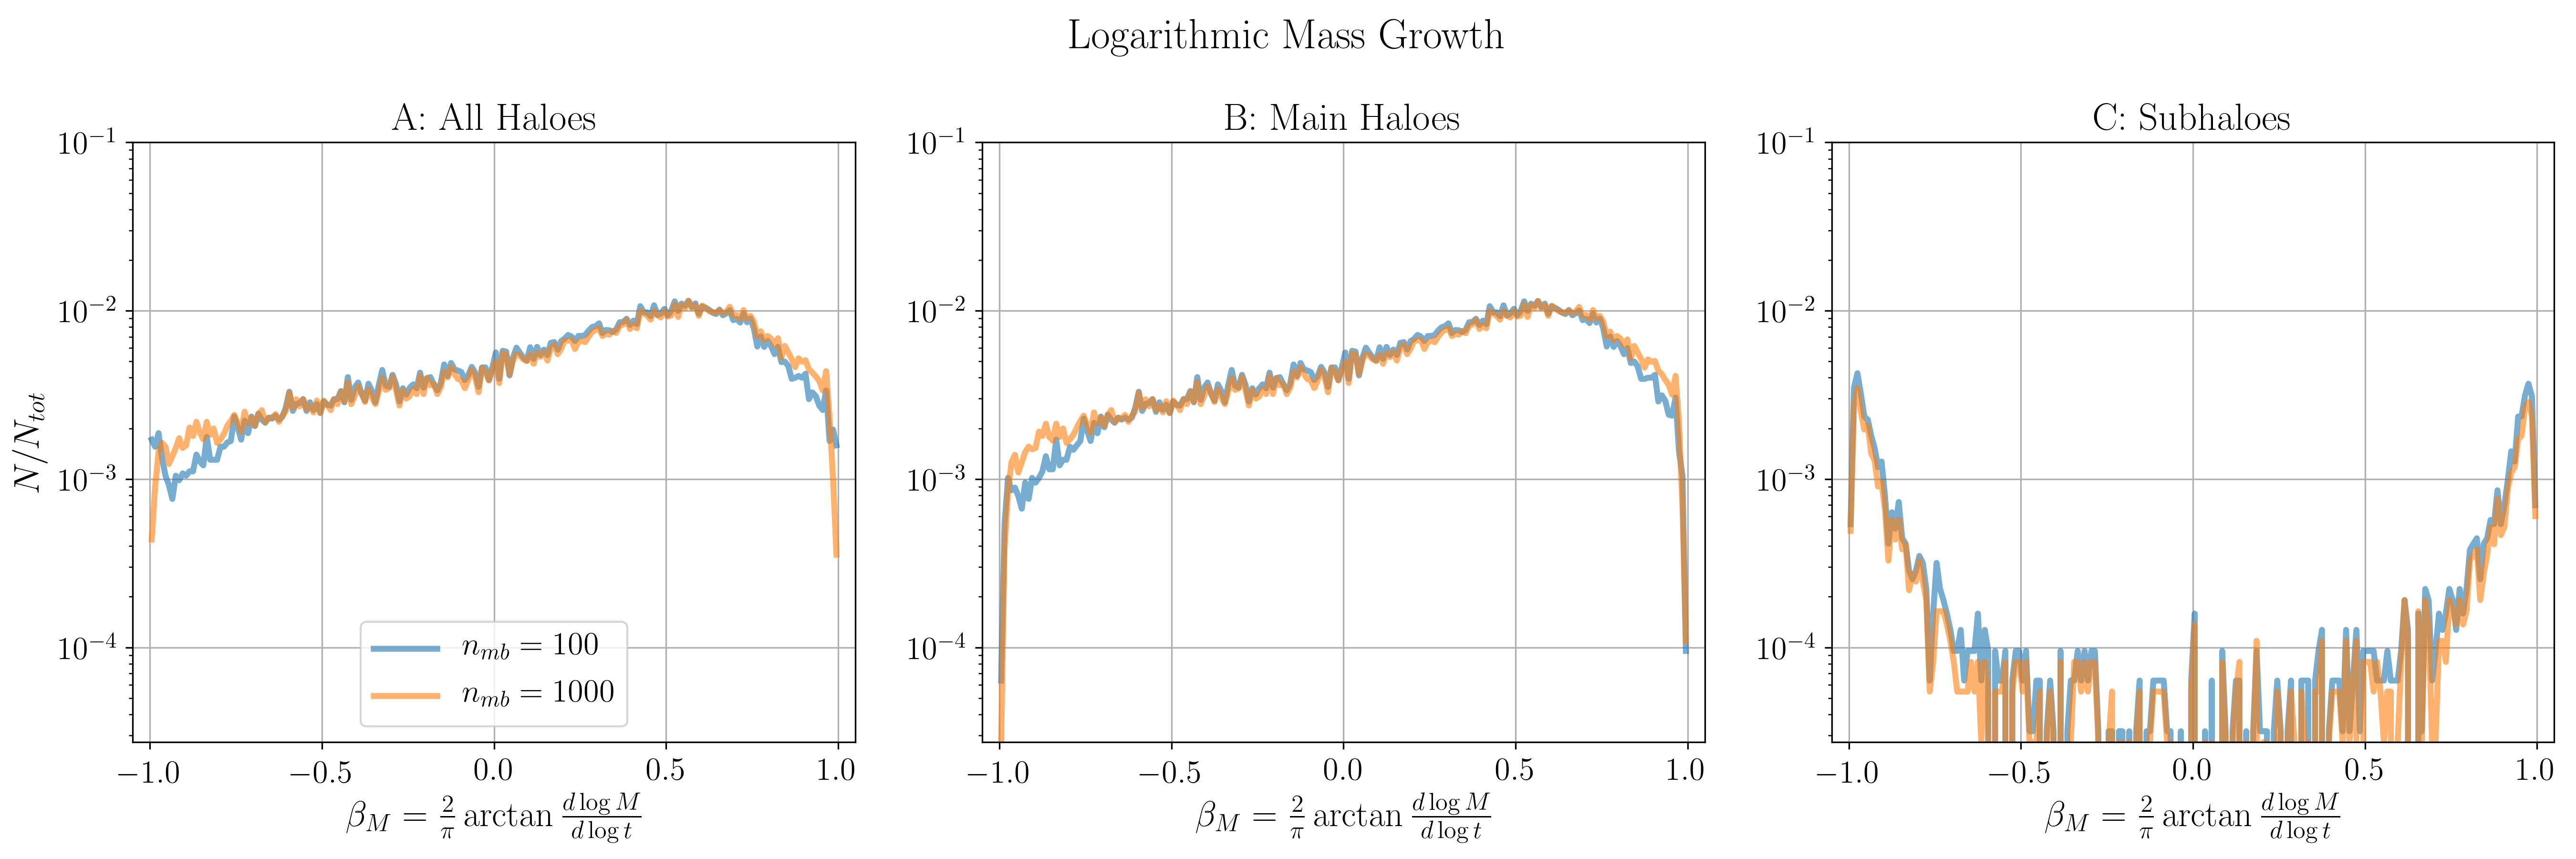
\includegraphics[width=\textwidth, keepaspectratio]{images/tree-statistics-sussing-threshold/mass_growth-ntrace.png}%
	\caption{
		Logarithmic mass growth for haloes and sub-haloes satisfying the mass thresholds.
		Group $A$ contains clumps that are either haloes or sub-haloes in consecutive snapshots $k$ and $k+1$ with masses $m \geq m_{m}$.
		Group $B$ contains clumps that are only haloes in two consecutive snapshots with mass above $m_{m}$, group $C$ contains only clumps that were sub-haloes in two consecutive snapshots with mass greater than $m_{s}$.
		The histogram is normalized by the total number of events found for group $A$.
	}%
	\label{fig:sussing-mass-growth}
\end{figure*}

\begin{figure*}
	\centering
	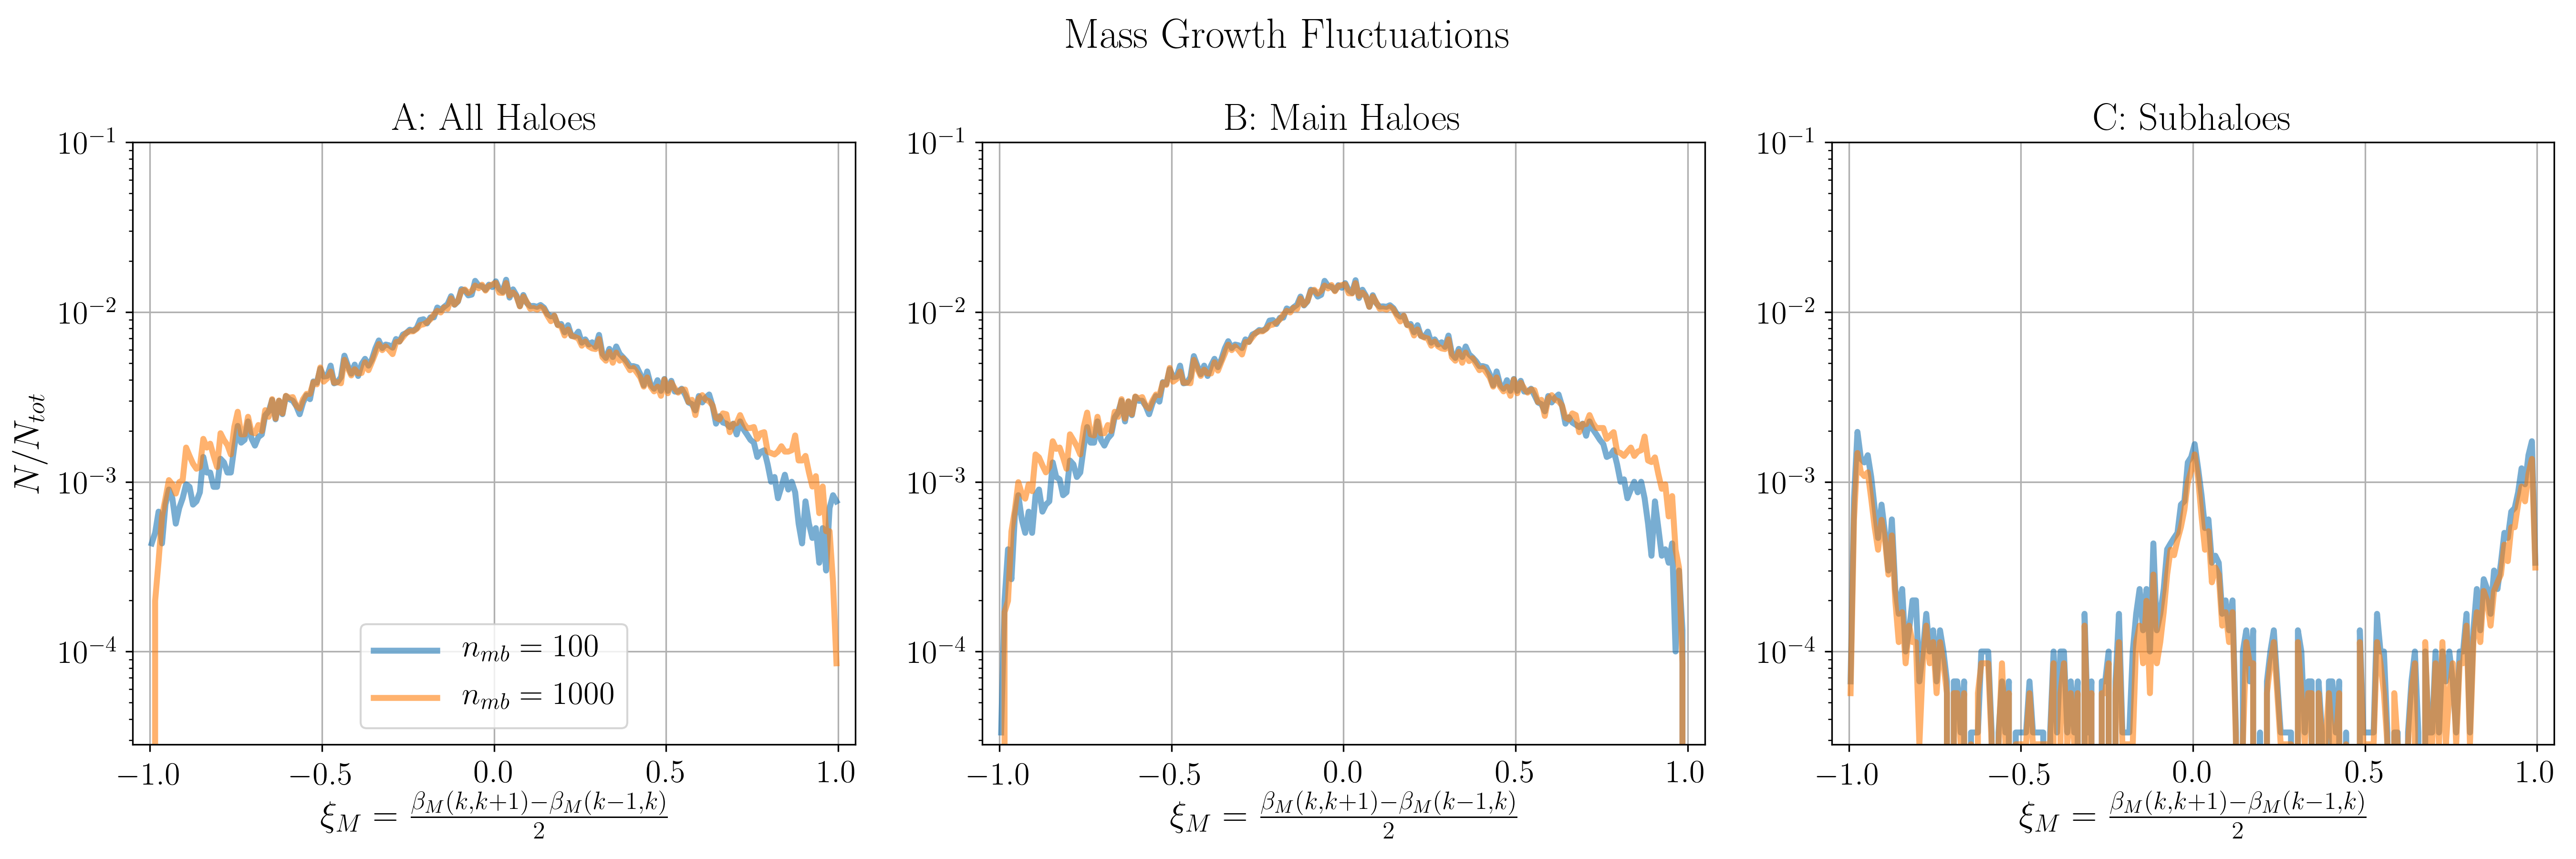
\includegraphics[width=\textwidth, keepaspectratio]{images/tree-statistics-sussing-threshold/mass_fluctuations-ntrace.png}\\%
	\caption{
		Histogram of mass growth fluctuations for haloes and sub-haloes satisfying the mass thresholds.
		Group $A$ contains clumps that are either haloes or sub-haloes in three consecutive snapshots with masses $m \geq m_{m}$.
		Group $B$ contains clumps that are only haloes in three consecutive snapshots with mass above $m_{m}$, group $C$ contains only clumps that were sub-haloes in three consecutive snapshots with mass greater than $m_{s}$.
		The histogram is normalized by the total number of events found for group $A$.
	}%
	\label{fig:sussing-mass-fluct}
\end{figure*}




In this section, the merger tree statistics introduced in Section \ref{chap:tests} when following the selection criteria that are used in \citet{SUSSING_HALOFINDER} (A14 from here on) are presented.
Ideally, \texttt{ACACIA} should be tested on the same datasets and halo catalogues used in the Comparison Project to enable a direct comparison to the performance of other merger tree codes. 
However, since \texttt{ACACIA} was designed to work on the fly, using it as a post-processing utility would defeat its purpose.
Furthermore, \texttt{ACACIA} is not necessarily compatible with other definitions of haloes and sub-haloes.
But most importantly, we also want to demonstrate that the halo finder \phew\ can be used to produce reliable merger trees. 
So instead, the tests are performed on our own datasets and halo catalogues, which are described in section \ref{chap:testing_methods}.
A comparison of the used parameters of our simulations and the ones used in A14 is given in Table \ref{tab:parameter-comparison}.
In the following, the results for $n_{mb} = 100$ and $n_{mb} = 1000$ are shown.
Like before, when the influence of the number of tracer particles was investigated, the \sad\ parameter and the \exc\ mass definition were used.


The difference to the results presented in Section \ref{chap:tests} is that the mass thresholds are set such that only the 1000 most massive main haloes and only the 200 most massive sub-haloes at $z = 0$ are included.
This gives effective mass threshold $m_{m} = 1.51 \times 10^{12} \msol$ and $m_{s} = 3.9 \times 10^{11}\msol$, which are on one hand comparable to the mass thresholds applied in A14 (Table \ref{tab:parameter-comparison}), but already show differences in the resulting halo catalogue.
\phew\ finds a higher mass threshold for main haloes, but a lower mass threshold for sub-haloes.
This is consistent with the fact that the \sad\ parameter was used:
Unbound particles are passed on to substructure that is higher up in the hierarchy, and the unbinding is repeated until the top level, which are the main haloes, is reached.
The more strict unbinding criterion tends to assign more particles to the main haloes and remove them from sub-haloes, which is reflected in the mass thresholds.
Indeed, using the \nosad\ parameter instead leads to $m_m = 1.39 \times 10^{12}\msol$ and $m_s = 2.00 \times 10^{12}\msol$.


The length of the main branches for haloes and sub-haloes individually are shown in Figure \ref{fig:sussing-branch-lengths}.
For the halo population, two noticeable differences compared to Figure 3 of A14 appear:
%
\begin{enumerate}
	\item \texttt{ACACIA} finds some main haloes with short (< 10) main branches.
	In A14, his only happens for the \texttt{JMerge} tree maker, \texttt{TreeMaker} for \texttt{Rockstar} haloes, and \texttt{SubLink} for \texttt{AHF} haloes. 
	\item Most clumps satisfying the mass thresholds have very large main branch lengths that are in a narrow range ($\sim 10$) of snapshots, while the high main branch length distribution found in A14 is much wider (> 20).
\end{enumerate}
%
This indicates that on one hand, \texttt{ACACIA} probably makes more misidentifications, hence the short main branches, but simultaneously is able to track clumps to higher redshifts.

In Figure \ref{fig:sussing-branching-ratio} the number of direct progenitors for all clumps between $z = 0$ and $z = 2$ are shown.
Comparing to Figure 5 of A14, \texttt{ACACIA} gives very comparable results:
$\sim 10^{-1}$ haloes have no direct progenitor, almost all have one, and the distribution follows an exponential decay with the maximal number of direct progenitors lying around 20-25.
Many tree makers and halo finders in A14 exhibit the same kind of behaviour, particularly so for the \texttt{AHF}, \texttt{Subfind}, and \texttt{Rockstar all} halo finders in Figure 5 of A14.



For the logarithmic mass growth (Figure \ref{fig:sussing-mass-growth}) and the mass growth fluctuations (Figure \ref{fig:sussing-mass-fluct}), the statistics are separated into three groups.
Group $A$ contains clumps that are either haloes or sub-haloes in \emph{consecutive} snapshots $k$ and $k+1$ with masses $m \geq m_{m}$.
Group $B$ contains clumps that are exclusively main haloes in two consecutive snapshots with mass above $m_{m}$, group $C$ contains only clumps that were sub-haloes in two consecutive snapshots with mass greater than $m_{s}$.
Except for the branching ratio statistic, we follow clumps of the $z = 0$ snapshot along the main branch only.

The logarithmic mass growth resulting from \texttt{ACACIA} follows the general trend that the tree makers in A14 exhibit too.
The growth for groups $A$ and $B$ increases steadily and peaks around $\beta_M \sim 0.5$, where the peak is $\sim 10^{-2}$.
For $n_{mb} = 100$, the extreme mass loss with $\beta_M = -1$ increases for group $A$, which is an undesirable property, but is also exhibited by \texttt{Sublink} in A14.
For $n_{mb} = 1000$, it drops below $10^{-3}$ ($10^{-4}$ for group $B$), which is comparable behaviour to \texttt{MergerTree}, \texttt{Sublink}, and \texttt{VELOCIraptor}, particularly so in combination with \texttt{AHF} and \texttt{Subfind} halo finders.
Group $C$, containing only mass growths of clumps that have been sub-haloes in two consecutive snapshots, shows a distribution peaking around extreme mass growths $\beta_M \rightarrow \pm 1$ at $\sim 5 \times 10^{-3}$, which can again be seen in A14 for almost all tree makers, albeit not for all halo finders.
More noticeably, almost no sub-haloes are found with $-0.5 < \beta_M < 0.5$ with \phew\ and \texttt{ACACIA} in Figure \ref{fig:sussing-mass-growth}.
This is most likely due to the fact that once a halo is merged into another, it quickly looses its outer mass due to to the strict unbinding method used here.
%Since only clumps that are identified as sub-haloes are included in group $C$, the statistics during the clump's lifetime as a halo are not included.

The mass growth fluctuations (Figure \ref{fig:sussing-mass-fluct}) of \texttt{ACACIA} share the general trend with the ones from Figure 8 in A14, in that they peak around $\xi_M = 0$ and decrease outwards towards $\xi_M = \pm 1$.
In A14, in all cases groups $A$ and $B$ peak just below $10^{-1}$, while our results peak just above $10^{-2}$.
However, similarly to the results of e.g. \texttt{Sublink}, \texttt{TreeMaker}, and \texttt{VELOCIraptor} with the \texttt{AHF} or \texttt{Subfind} halo finders, the distribution around $\xi_M \sim \pm 0.5$ drops to $\sim 5 \times 10^{-3}$, and then continues dropping below $10^{-4} - 10^{-3}$ at $\xi_M \sim \pm 1$.
For $n_{mb} = 100$, the group $A$ distribution rises again for $\xi_M \sim 1$, as it does for \texttt{TreeMaker} and \texttt{Sublink} tree makers with \texttt{AHF}.
Group $B$ shows a steeper drop around the extreme values $\xi_M \sim \pm 1$ compared to group $A$, dropping below $10^{-4}$ at these values, similarly to the behaviour of many tree makers and halo finders in A14.
The sub-halo group $C$ of this work shows three main peaks, around $-1$, $0$, and $1$.
These peaks also appear in the A14 results.
However, the peaks at the extreme values in A14 are lower than the ones of this work, while the peaks around $0$ is higher.
The missing values around $\xi_M \sim \pm 0.5$ that were also seen in the mass growth in Figure \ref{fig:sussing-mass-growth} remain unsurprisingly.
Similar distributions are obtained by \texttt{Sublink} and \texttt{VELOCIraptor} in combination with the \texttt{AHF} halo finder.




In summary:

\begin{enumerate}
	\item \texttt{ACACIA} finds more massive haloes with short main branch lengths, but the main branch length distribution peaks at very high numbers and is narrower
	\item The distribution of the number of direct progenitors for all haloes within $0 < z < 2$ is consistent with the results from A14
	\item The logarithmic mass growth is similar to what is obtained with some other halo finders and tree makers, in particular the \texttt{Sublink} and \texttt{VELOCIraptor} tree makers in combination with the \texttt{AHF} and \texttt{Subfind} halo finders. 
	\item Apart of the higher peak value of the distribution in A14, the mass growth fluctuations are similar to the results of the \texttt{Sublink} and \texttt{VELOCIraptor} tree makers in combination with the \texttt{AHF} halo finder.
\end{enumerate}

Hence we conclude that our tree maker gives comparable results with respect to other state of the art merger tree and halo finding codes.